\documentclass[a4paper,10pt,twocolumn,department=FakEI]{OTHRartcl}

% ==============================================================================
% Pakete und Grundeinstellungen
% ==============================================================================
\usepackage[utf8]{inputenc}
\usepackage[T1]{fontenc}
\usepackage[ngerman]{babel}
\usepackage[left=13mm,right=13mm,top=22mm,bottom=20mm,headsep=6mm,footskip=8mm]{geometry}

\usepackage{amsmath}
\usepackage{amssymb}
\usepackage{amsfonts}
\usepackage{mathtools}
\usepackage{bm}

\usepackage{graphicx}
\usepackage{tcolorbox}
\tcbuselibrary{skins,breakable}

\usepackage{booktabs}
\usepackage{array}
\usepackage{tabularx}
\usepackage{multirow}
\usepackage{listings}
\usepackage{xcolor}

\usepackage[headsepline]{scrlayer-scrpage}
\usepackage{lastpage}
\usepackage{hyperref}

% ==============================================================================
% Farb- und Box-Definitionen (exakt wie in der Vorlage main-3)
% ==============================================================================
\tcbset{
  colback=black!6,
  colframe=black!6,
  arc=2.5mm,
  boxrule=0pt,
  left=4pt,
  right=4pt,
  top=3.5pt,
  bottom=3.5pt,
  boxsep=1pt
}

% Eigene Formelbox mit horizontalem Trennstrich bei Titeln
\newcommand{\boxtitle}[1]{\textbf{#1}\par\vspace{1.5pt}\hrule height 0.4pt\vspace{3.5pt}}

% Listings für C-Code / Algorithmen
\lstset{
  language=C,
  basicstyle=\ttfamily\scriptsize,
  keywordstyle=\bfseries\color{blue!70!black},
  commentstyle=\color{green!50!black}\itshape,
  stringstyle=\color{red!70!black},
  numbers=left,
  numberstyle=\tiny\color{gray},
  stepnumber=1,
  numbersep=4pt,
  frame=single,
  rulecolor=\color{black!15},
  backgroundcolor=\color{black!4},
  tabsize=2,
  breaklines=true,
  breakatwhitespace=false,
  showspaces=false,
  showstringspaces=false
}

% ==============================================================================
% Kopf- und Fußzeilen (Scrlayer-Scrpage)
% ==============================================================================
\clearpairofpagestyles
\ihead{\textsf{Johannes Wutz}}
\ohead{\textsf{\rightmark}}
\cfoot{\textsf{\thepage\ von \pageref{LastPage}}}
\setheadsepline{0.4pt}
\pagestyle{scrheadings}
\automark[section]{section}
\automark*[subsection]{}

% Hyperref Setup
\hypersetup{
  colorlinks=false,
  pdfborder={0 0 0},
  pdftitle={Formelsammlung Regelungstechnik (RT & RTA)},
  pdfauthor={Johannes Wutz}
}

% ==============================================================================
% Dokumentbeginn
% ==============================================================================
\begin{document}

% ------------------------------------------------------------------------------
% Deckblatt (einspaltig im OTHR CI-Design)
% ------------------------------------------------------------------------------
\onecolumn
\thispagestyle{empty}

\begin{center}
  \vspace*{1.5cm}
  
\includegraphics[width=0.48\textwidth]{images/othr_logo.png}
  
  \vspace{3.5cm}
  
  {\Huge \textsc{Formelsammlung}}\\[1.2em]
  {\Huge \textbf{Regelungstechnik}}\\[0.6em]
  {\LARGE \textbf{(RT \& RTA)}}\\[2.5em]
  
  {\large nach Vorlesungsunterlagen von}\\[0.5em]
  {\Large \textbf{Prof. Dr.-Ing. Claus Brüdigam}}\\[0.8em]
  {\large Ostbayerische Technische Hochschule Regensburg}\\[0.3em]
  {\large Fakultät Elektro- und Informationstechnik}
  
  \vfill
  
  \begin{tabular}{ll}
    \textbf{Originalversion:} & Maximilian Binninger \\
    \textbf{Überarbeitet:} & Bastian Nagler \\
    \textbf{Erweitert (RT \& RTA):} & Johannes Wutz \\
    \textbf{Letzter Stand:} & WS 2025/26 \\
    \textbf{Lizenz:} & GPLv3 \\
  \end{tabular}
  \vspace*{1.5cm}
\end{center}

\newpage

% ------------------------------------------------------------------------------
% Inhaltsverzeichnis (einspaltig)
% ------------------------------------------------------------------------------
\thispagestyle{empty}
\tableofcontents
\newpage

% ------------------------------------------------------------------------------
% Hauptteil (zweispaltig)
% ------------------------------------------------------------------------------
\twocolumn
\setcounter{page}{1}

\section{Grundlagen}

\subsection{Gleichungen zur Modellbildung}

\begin{tcolorbox}
\boxtitle{Kräftegleichungen (Translation)}
Federkraft: $F_F = k_F \cdot x$\\[2pt]
Dämpferkraft: $F_D = k_D \cdot v = k_D \cdot \dot{x}$\\[2pt]
Trägheitskraft: $F_{Tr} = m \cdot a = m \cdot \ddot{x}$\\[2pt]
Erdanziehungskraft: $F_G = m \cdot g$
\end{tcolorbox}

\begin{tcolorbox}
\boxtitle{Momentengleichungen (Rotation)}
Widerstandsmoment: $M_W = k_D \cdot \omega$\\[2pt]
Trägheitsmoment: $M_{Tr} = J \cdot \dot{\omega} = J \cdot \ddot{\varphi}$
\end{tcolorbox}

\begin{tcolorbox}
\boxtitle{Elektrischer Grundkreis (RLC)}
\[
u(t) = L \cdot \frac{di}{dt} + R \cdot i + \frac{1}{C} \int i \, dt
\]
\end{tcolorbox}

\begin{tcolorbox}
\boxtitle{Rotation in Flüssigkeit}
\[
M = M_{\text{Träg}} + M_{\text{Brems}} = J \cdot \dot{\omega} + k_{\text{Flüssigkeit}} \cdot \omega
\]
\end{tcolorbox}

\subsection{Mathematische Grundlagen}
\begin{tcolorbox}
\boxtitle{Kleine Winkel}
Für kleine Winkel $\alpha$ (im Bogenmaß) gilt:\\[2pt]
$\sin(\alpha) \approx \alpha, \quad \tan(\alpha) \approx \alpha, \quad \cos(\alpha) \approx 1 - \frac{\alpha^2}{2} \approx 1$
\end{tcolorbox}

\begin{tcolorbox}
\boxtitle{Grenzwertsätze der Laplace-Transformation}
\textbf{Anfangswertsatz:}\\[2pt]
\[
x(t \to +0) = \lim_{s \to \infty} s \cdot X(s)
\]
\textbf{Endwertsatz:}\\[2pt]
\[
x(t \to \infty) = \lim_{s \to 0} s \cdot X(s)
\]
\textbf{Gültigkeitsbedingung:} Der Endwertsatz gilt \textbf{nur}, wenn höchstens ein Pol von $s \cdot X(s)$ im Ursprung liegt und alle anderen Pole in der offenen linken $s$-Halbebene liegen ($\text{Re}\{s_P\} < 0$).
\end{tcolorbox}

\subsection{Linearisierung um den Arbeitspunkt}
\begin{tcolorbox}
Nichtlineare Kennlinie $x_a = f(x_{e1}, \dots, x_{en})$ um den stationären Arbeitspunkt $AP = (x_{e1,AP}, \dots, x_{en,AP})$:
\begin{align*}
x_a(t) &= x_{a,AP} + \Delta x_a(t) \\
&\approx f(x_{e1,AP}, \dots, x_{en,AP}) + \sum_{m=1}^n \left. \frac{\partial f}{\partial x_{em}} \right|_{AP} \cdot \Delta x_{em}(t)
\end{align*}
Lineare Kleinsignalbeziehung für die Abweichungen:
\[
\Delta x_a(t) \approx \sum_{m=1}^n K_m \cdot \Delta x_{em}(t) \quad \text{mit } K_m = \left. \frac{\partial f}{\partial x_{em}} \right|_{AP}
\]
\end{tcolorbox}

\subsection{Eigenschaften von LTI-Systemen}
\begin{tcolorbox}
\begin{enumerate}
  \item \textbf{BIBO-Stabilität} (Bounded Input / Bounded Output):
  \[
  |y(t)| < \infty \quad \text{für } |x(t)| < \infty
  \]
  \item \textbf{Linearität} (Superposition und Homogenität):
  \[
  f\left\{ \sum_{n=1}^N a_n x_n(t) \right\} = \sum_{n=1}^N a_n f\{x_n(t)\}
  \]
  \item \textbf{Zeitinvarianz}:
  \[
  f\{x(t - t_0)\} = y(t - t_0)
  \]
  \item \textbf{Kausalität}: Das System reagiert nicht vor Eintreffen des Eingangssignals:
  \[
  x(t) = 0 \text{ für } t < 0 \implies y(t) = 0 \text{ für } t < 0
  \]
\end{enumerate}
\end{tcolorbox}

\subsection{Systemantworten}
\begin{tcolorbox}
\boxtitle{Sprungantwort ($x(t) = \sigma(t)$)}
\[
g(t) = \mathcal{L}^{-1}\{G(s)\} = \mathcal{L}^{-1}\left\{ \frac{F(s)}{s} \right\} = \int_0^t h(\tau) \, d\tau
\]
\end{tcolorbox}

\begin{tcolorbox}
\boxtitle{Impulsantwort ($x(t) = \delta(t)$)}
\[
h(t) = \int_{-\infty}^\infty x(\tau) \delta(t - \tau) \, d\tau = \mathcal{L}^{-1}\{F(s)\} = \frac{d}{dt} g(t)
\]
\end{tcolorbox}

\subsection{Abtasttheorem}
\begin{tcolorbox}
Durch die periodische Abtastung eines Signals $f(t)$ mit der Periode $T_A$ (bzw. $\omega_A = 2\pi/T_A$) wird das kontinuierliche Spektrum $F(\omega)$ unendlich oft um die Vielfachen der Abtastkreisfrequenz reproduziert:
\[
F_A(\omega) = \frac{1}{T_A} \sum_{n=-\infty}^\infty F(\omega - n \omega_A)
\]
\textbf{Shannon/Nyquist-Bedingung:}\\[2pt]
Zur fehlerfreien (aliasingfreien) Rekonstruktion muss die Abtastfrequenz mindestens doppelt so groß wie die höchste Grenzfrequenz $\omega_g$ des abzutastenden Signals sein:
\[
\omega_A \ge 2 \omega_g \quad \text{bzw.} \quad f_A \ge 2 f_g
\]
\end{tcolorbox}

\section{Systemtechnik}

\subsection{Modellbildung}
\begin{tcolorbox}
\boxtitle{Hinweise zum Aufstellen der Differentialgleichung (DGL)}
\begin{enumerate}
  \item \textbf{Bestimmung} der Ein- und Ausgangsgrößen.
  \item \textbf{Suche} nach dem beschreibenden physikalischen Gleichgewicht (Kräfte-, Momenten-, Knoten-, Maschenbilanz).
  \item In der Endgleichung dürfen nur Konstanten sowie die Ein- und Ausgangsgrößen in beliebiger Zeitableitung vorkommen.
  \item Alle Zwischenvariablen müssen durch physikalische Gesetze eliminiert werden.
\end{enumerate}
\end{tcolorbox}

\subsection{Signalflussplan / Blockschaltbild}
\begin{tcolorbox}
\boxtitle{Erzeugung des Signalflussplans aus der DGL}
\begin{enumerate}
  \item Für technische Realisierbarkeit gilt: $m \le n$ (Zählergrad $\le$ Nennergrad).
  \item DGL nach der höchsten Ableitung der Ausgangsgröße auflösen.
  \item Die höchste Ableitung der Ausgangsgröße wird auf den Eingang einer Kette von $n$ Integratoren ($1/s$) geführt.
\end{enumerate}
\end{tcolorbox}

\begin{center}
  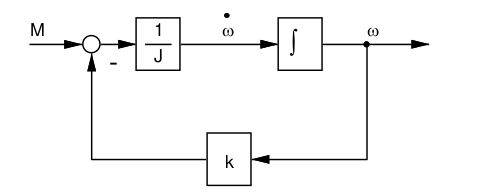
\includegraphics[width=0.95\columnwidth]{images/sfp_dgl_masse_feder.png}
\end{center}

\begin{tcolorbox}
\boxtitle{Signalflussplan eines Systems $n$-ter Ordnung mit DGL:}
\[
a_n x_a^{(n)} + \dots + a_1 \dot{x}_a + a_0 x_a = b_m x_e^{(m)} + \dots + b_1 \dot{x}_e + b_0 x_e
\]
\begin{center}
  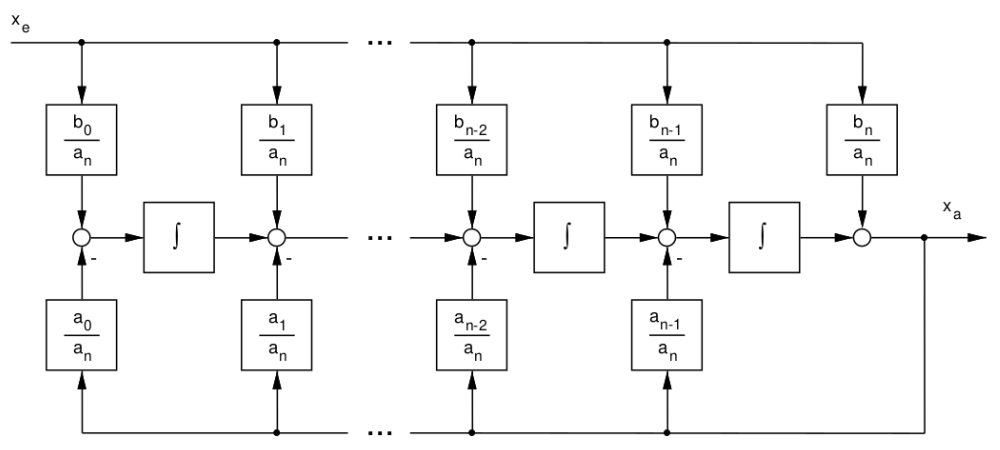
\includegraphics[width=\columnwidth]{images/sfp_dgl_ordnung.png}
\end{center}
Falls $m < n$, sind alle höheren Koeffizienten $b_\mu = 0$ zu setzen.
\end{tcolorbox}

\subsection{Übertragungsfunktion $F(s)$}
\begin{tcolorbox}
Definition bei verschwindenden Anfangsbedingungen:
\[
F(s) = \frac{\mathcal{L}\{x_a(t)\}}{\mathcal{L}\{x_e(t)\}} = \frac{X_a(s)}{X_e(s)}
\]
\end{tcolorbox}

\subsubsection{$F(s)$ aus der DGL}
\begin{tcolorbox}
\[
F(s) = \frac{b_m s^m + b_{m-1} s^{m-1} + \dots + b_1 s + b_0}{a_n s^n + a_{n-1} s^{n-1} + \dots + a_1 s + a_0}
\]
\end{tcolorbox}

\subsubsection{$F(s)$ in Pol- und Nullstellenform}
\begin{tcolorbox}
\[
F(s) = Q \cdot \frac{\prod_{\mu=1}^m (s - s_{N\mu})}{\prod_{\nu=1}^n (s - s_{P\nu})} \quad \text{mit } Q = \frac{b_m}{a_n}
\]
\textbf{Eigenschaften von Polen ($s_{P\nu}$):}
\begin{itemize}
  \item Pole in der rechten $s$-Halbebene ($\text{Re}\{s_P\} > 0$) führen zu einem \textbf{instabilen} System. Sie können \textbf{nicht} durch Nullstellen kompensiert werden!
  \item Pole bewirken verzögerndes Verhalten. Je weiter links sie in der komplexen Ebene liegen, desto schneller klingt der Einschwingvorgang ab.
  \item Liegen Pole deutlich weiter links als dominante Pole, können sie meist ohne großen Fehler vernachlässigt werden.
\end{itemize}
\textbf{Eigenschaften von Nullstellen ($s_{N\mu}$):}
\begin{itemize}
  \item Nullstellen bewirken differenzierendes Verhalten (Vorhalt, Phasendrehung nach oben, Beschleunigung des Systems).
  \item Nullstellen weit links in der $s$-Ebene haben geringen Einfluss.
\end{itemize}
\end{tcolorbox}

\subsection{Signalflussplan-Algebra}

\begin{tcolorbox}
\boxtitle{Kettenstruktur (Reihenschaltung)}
\begin{center}
  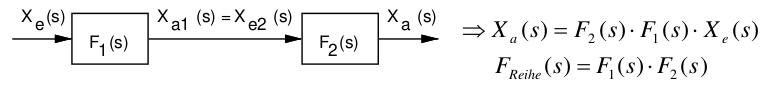
\includegraphics[width=0.9\columnwidth]{images/sfp_reihe.png}
\end{center}
\[
X_a(s) = F_2(s) \cdot F_1(s) \cdot X_e(s) \implies F_{\text{Reihe}}(s) = F_1(s) \cdot F_2(s)
\]
\end{tcolorbox}

\begin{tcolorbox}
\boxtitle{Parallelstruktur (Parallelschaltung)}
\begin{center}
  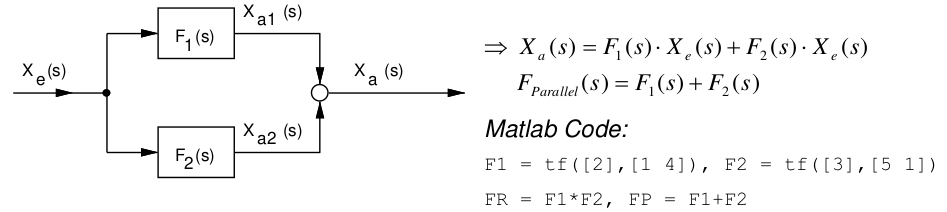
\includegraphics[width=0.9\columnwidth]{images/sfp_parallel.png}
\end{center}
\[
F_{\text{Parallel}}(s) = F_1(s) + F_2(s)
\]
\end{tcolorbox}

\begin{tcolorbox}
\boxtitle{Kreisstruktur (Rückkopplung)}
\begin{center}
  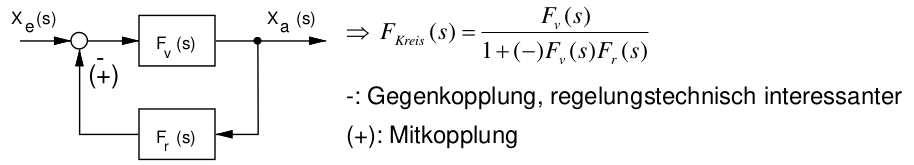
\includegraphics[width=0.75\columnwidth]{images/sfp_kreis.png}
\end{center}
\[
F_{\text{Kreis}}(s) = \frac{F_v(s)}{1 + F_v(s) \cdot F_r(s)} \quad \text{bei Gegenkopplung (-)}
\]
(Bei Mitkopplung (+) steht im Nenner $1 - F_v(s) F_r(s)$).
\end{tcolorbox}

\begin{tcolorbox}
\boxtitle{Verschieben einer Additionsstelle}
\begin{center}
  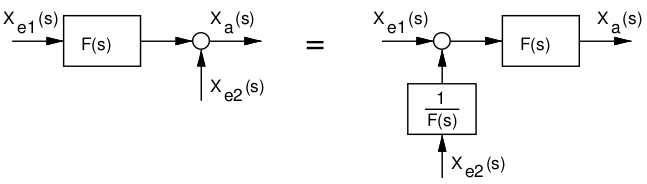
\includegraphics[width=\columnwidth]{images/sfp_addition_verschieben.png}
\end{center}
\end{tcolorbox}

\begin{tcolorbox}
\boxtitle{Verschieben einer Verzweigung}
\begin{center}
  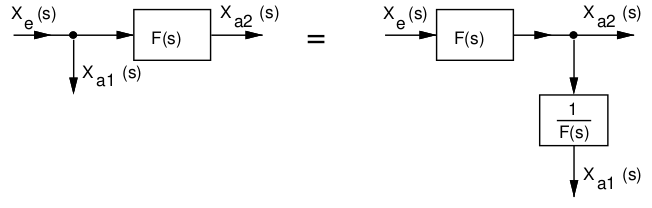
\includegraphics[width=\columnwidth]{images/sfp_verzweigung_verschieben.png}
\end{center}
\end{tcolorbox}

\subsection{Standard-Übertragungsglieder}
\begin{tcolorbox}
\small
\begin{tabularx}{\columnwidth}{l X X}
\toprule
\textbf{Typ} & \textbf{Übertragungsfunktion $F(s)$} & \textbf{Sprungantwort $h(t)$} \\
\midrule
\textbf{P} & $K_P$ & $K_P \cdot \sigma(t)$ \\[2pt]
\textbf{I} & $\frac{K_I}{s} = \frac{1}{T_I s}$ & $K_I \cdot t = \frac{t}{T_I}$ \\[2pt]
\textbf{D} & $K_D \cdot s = T_D s$ & $K_D \cdot \delta(t)$ \\[2pt]
\textbf{PT}$_1$ & $\frac{K}{1 + T s}$ & $K (1 - e^{-t/T})$ \\[2pt]
\textbf{PT}$_2$ & $\frac{K}{1 + \frac{2D}{\omega_0} s + \frac{s^2}{\omega_0^2}}$ & $K \left[1 - \frac{e^{-D\omega_0 t}}{\sqrt{1-D^2}} \sin(\omega_d t + \varphi)\right]$ \\[2pt]
\textbf{IT}$_1$ & $\frac{K_I}{s (1 + T s)}$ & $K_I [t - T(1 - e^{-t/T})]$ \\[2pt]
\textbf{DT}$_1$ & $\frac{K_D s}{1 + T s}$ & $\frac{K_D}{T} e^{-t/T}$ \\[2pt]
\textbf{T}$_t$ & $e^{-s T_t}$ & $\sigma(t - T_t)$ \\
\bottomrule
\end{tabularx}
\end{tcolorbox}

\section{Zusammenwirken mehrerer Systeme (Analoge Regelung)}

\subsection{Regelkreis}
\begin{tcolorbox}
\boxtitle{Wichtige Begriffe und Signalbezeichnungen}
\begin{itemize}
  \item \textbf{Führungsgröße:} $w(t)$ (Sollwert)
  \item \textbf{Störgrößen:} $z(t)$ bzw. $z_1(t), z_2(t), z_3(t)$
  \item \textbf{Regelgröße:} $x(t)$ (Istwert)
  \item \textbf{Stellgröße:} $y(t)$ bzw. $u(t)$ (Reglerausgang)
  \item \textbf{Regeldifferenz / Regelabweichung:} $e(t) = w(t) - x(t)$
  \item \textbf{Maximale Überschwingweite:} $h_{\max}$ (maximale Regelabweichung nach erstmaligem Erreichen des Sollwertes)
  \item \textbf{Anregelzeit $t_{\text{an}}$:} Zeit bis zum erstmaligen Erreichen des Sollwertes
  \item \textbf{Ausregelzeit $t_{\text{aus}}$:} Zeit bis zum dauerhaften Verbleib im vorgegebenen Toleranzband (z.\,B. $\pm 2\%$ oder $\pm 5\%$)
\end{itemize}
\end{tcolorbox}

\begin{tcolorbox}
\boxtitle{Anforderungen an den Regelkreis}
\begin{itemize}
  \item \textbf{Stabilität:} Der geschlossene Regelkreis muss stabil sein (auch bei grenzstabilen oder instabilen Strecken).
  \item \textbf{Gutes Führungsverhalten:} Kleines oder kein Überschwingen, schnelle Ausregelung, keine bleibende Regelabweichung.
  \item \textbf{Gutes Störverhalten:} Rasche Dämpfung und Unterdrückung von äußeren Störungen $z(t)$.
\end{itemize}
\end{tcolorbox}

\begin{tcolorbox}
\boxtitle{Grundstruktur des einschleifigen Regelkreises}
\begin{center}
  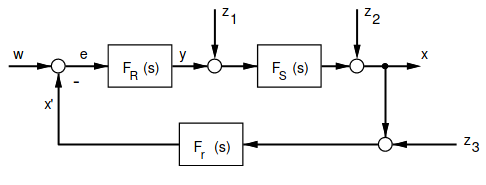
\includegraphics[width=\columnwidth]{images/regelkreis_grundstruktur.png}
\end{center}
Überlagerung der Einflüsse auf die Regelgröße $X(s)$:
\[
X(s) = \frac{F_v}{1 + F_v F_r} W(s) + \frac{1}{1 + F_v F_r} Z_1(s) - \frac{F_v F_r}{1 + F_v F_r} Z_2(s)
\]
Mit $F_0(s) = F_R(s) \cdot F_S(s) \cdot F_r(s)$ (Frequenzgang des offenen Kreises) und $F_r(s) = 1$ (Einheitsrückführung):
\begin{align*}
F_w(s) &= \frac{F_R(s) F_S(s)}{1 + F_0(s)} \quad \text{(Führungsübertragungsfunktion)} \\
F_{z1}(s) &= \frac{1}{1 + F_0(s)} \quad \text{(Störübertragungsfunktion 1)} \\
F_{z2}(s) &= \frac{-F_S(s) F_r(s)}{1 + F_0(s)} \quad \text{(Störübertragungsfunktion 2)}
\end{align*}
\end{tcolorbox}

\subsection{Wurzelortskurven (WOK)-Verfahren}
\begin{tcolorbox}
Aufspaltung der Reglerübertragungsfunktion in Verstärkung $K$ und Reglerdynamik $F_R'(s)$:
\[
F_R(s) = K \cdot F_R'(s) \implies F_0(s) = K \cdot Q \cdot \frac{\prod_{\mu=1}^m (s - s_{N0\mu})}{\prod_{\nu=1}^n (s - s_{P0\nu})}
\]
Pole des geschlossenen Regelkreises erfüllen die charakteristische Gleichung:
\[
1 + F_0(s) = 0 \implies F_0(s) = -1
\]
Aufteilung in Betrags- und Phasenbedingung:
\begin{align*}
\textbf{Betrag:} \quad &\frac{\prod_{\nu=1}^n |s - s_{P0\nu}|}{\prod_{\mu=1}^m |s - s_{N0\mu}|} = |K \cdot Q| \\
\textbf{Phase:} \quad &\sum_{\nu=1}^n \angle(s - s_{P0\nu}) - \sum_{\mu=1}^m \angle(s - s_{N0\mu}) = \pm r \cdot 180^\circ
\end{align*}
wobei $r = 1, 3, 5, \dots$ für $K \cdot Q > 0$ und $r = 0, 2, 4, \dots$ für $K \cdot Q < 0$.
\end{tcolorbox}

\begin{tcolorbox}
\boxtitle{Konstruktionsregeln für die WOK}
\begin{enumerate}
  \item \textbf{Startpunkte:} Die $n$ Äste der WOK beginnen für $K = 0$ in den $n$ Polen $s_{P0\nu}$ des offenen Kreises.
  \item \textbf{Endpunkte:} $m$ Äste enden für $K \to \infty$ in den $m$ Nullstellen $s_{N0\mu}$.
  \item \textbf{Asymptoten:} $n - m$ Äste (Polüberschuss) streben für $K \to \infty$ ins Unendliche.
  \item \textbf{Asymptotengeometrie:}
  \begin{itemize}
    \item Wurzelschwerpunkt (Schnittpunkt auf der reellen Achse):
    \[
    s_w = \frac{\sum_{\nu=1}^n s_{P0\nu} - \sum_{\mu=1}^m s_{N0\mu}}{n - m}
    \]
    \item Asymptotenwinkel mit der positiven reellen Achse:
    \[
    \varphi_k = \frac{(2k - 1) \cdot 180^\circ}{n - m} \quad (k = 1, \dots, n-m \text{ bei } KQ > 0)
    \]
  \end{itemize}
  \item \textbf{Symmetrie:} Die WOK ist spiegelsymmetrisch zur reellen Achse.
  \item \textbf{Reelle Achse:} Ein Punkt auf der reellen Achse gehört zur WOK, wenn rechts von ihm eine \textbf{ungerade} Anzahl reeller Pole und Nullstellen liegt (bei $KQ > 0$).
\end{enumerate}
\textbf{Stabilitätsgrenze:} Schnittpunkte der WOK mit der Imaginärachse liefern $s_{\text{krit}} = j\omega_{\text{krit}}$. Einsetzen in die Betragsbedingung ergibt die kritische Verstärkung $K_{\text{krit}}$.
\end{tcolorbox}

\subsection{Nyquist-Kriterium}
\begin{tcolorbox}
Frequenzgang des offenen Regelkreises: $F_0(j\omega) = F_R(j\omega) F_S(j\omega) F_r(j\omega)$.\\[2pt]
\textbf{Schwingbedingung:}
\[
F_0(j\omega_{\text{krit}}) = -1 = 1 \cdot e^{-j 180^\circ}
\]
Die Schwingbedingung ist erfüllt, wenn die Ortskurve von $F_0(j\omega)$ durch den kritischen Punkt $P_{\text{krit}} = -1 + j0$ verläuft.
\end{tcolorbox}

\begin{tcolorbox}
\boxtitle{Vereinfachtes Nyquist-Kriterium (Linke-Hand-Regel)}
Voraussetzung: Die offene Übertragungsfunktion $F_0(s)$ besitzt \textbf{keine} Pole in der rechten $s$-Halbebene und maximal zwei Pole im Ursprung ($s=0$).\\[3pt]
\textbf{Kriterium:} Der geschlossene Regelkreis ist genau dann \textbf{asymptotisch stabil}, wenn beim Durchlaufen der Ortskurve von $F_0(j\omega)$ in Richtung wachsender Frequenz ($\omega = 0 \to \infty$) der kritische Punkt $P_{\text{krit}} = -1 + j0$ stets \textbf{zur Linken} liegt.
\end{tcolorbox}

\begin{tcolorbox}
\boxtitle{Stabilität im Bode-Diagramm}
Bei minimalphasigen Strecken ist der Regelkreis stabil, wenn die Durchtrittsfrequenz $\omega_{A=1}$ kleiner ist als die Phasenschnittfrequenz $\omega_{\varphi=-180^\circ}$:
\[
\omega_{A=1} < \omega_{\varphi=-180^\circ}
\]
\textbf{Stabilitätsränder:}
\begin{itemize}
  \item \textbf{Phasenrand (Phasenreserve):}
  \[
  \varphi_R = \varphi(\omega_{A=1}) - (-180^\circ) = \varphi(\omega_{A=1}) + 180^\circ
  \]
  \item \textbf{Amplitudenrand (Verstärkungsreserve):}
  \[
  A_R = \frac{1}{|F_0(j\omega_{\varphi=-180^\circ})|} \quad \text{bzw.} \quad A_{R,\text{dB}} = -20 \lg |F_0(j\omega_{\varphi=-180^\circ})|
  \]
\end{itemize}
\end{tcolorbox}

\begin{center}
  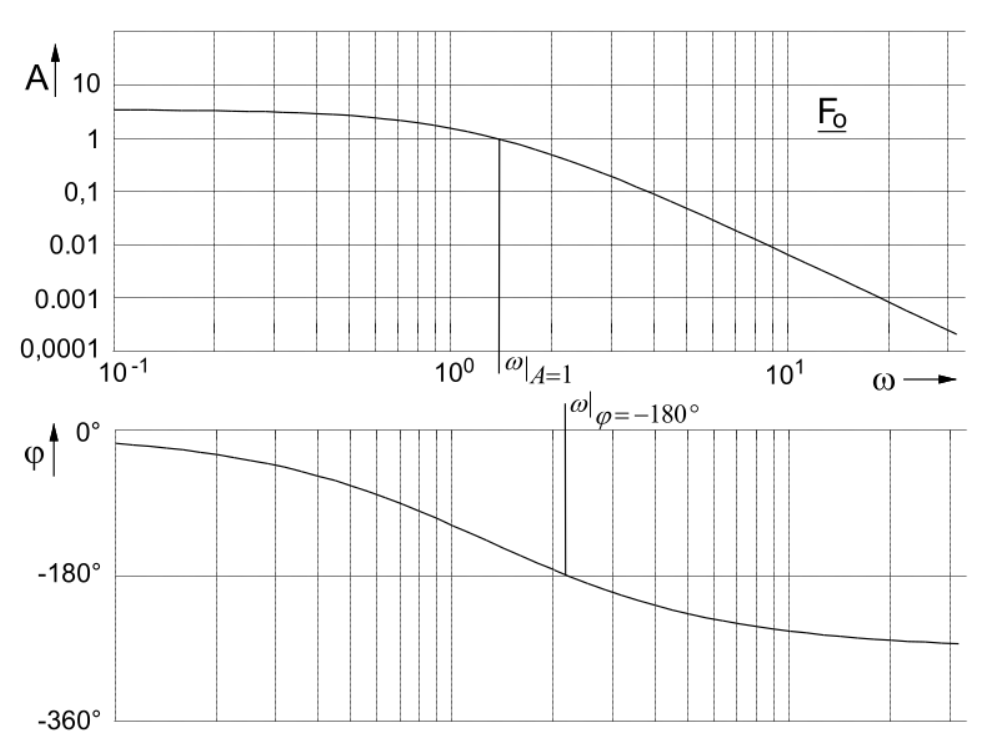
\includegraphics[width=0.9\columnwidth]{images/bode_raender.png}
\end{center}

\begin{tcolorbox}
\boxtitle{Allgemeines Nyquist-Kriterium}
Gilt auch für instabile offene Systeme. Der geschlossene Kreis ist stabil, wenn der Fahrstrahl von $P_{\text{krit}} = -1+j0$ zur Ortskurve $F_0(j\omega)$ für $\omega = +0 \to +\infty$ eine Winkeländerung von
\[
\Delta \varphi_{\text{soll}} = n_r \cdot 180^\circ + n_a \cdot 90^\circ
\]
im mathematisch positiven Sinn (gegen den Uhrzeigersinn) erfährt.
\begin{itemize}
  \item $n_r$: Anzahl der Pole des offenen Kreises in der rechten $s$-Halbebene.
  \item $n_a$: Anzahl der Pole auf der imaginären Achse (ohne Ursprung).
\end{itemize}
\end{tcolorbox}

\subsection{Reglerauslegung im Bode-Diagramm}
\begin{tcolorbox}
\begin{itemize}
  \item \textbf{Kleine bleibende Regeldifferenz:} $A(\omega) \gg 1$ bei tiefen Frequenzen ($\omega \ll \omega_{A=1}$).
  \item \textbf{Stabilität:} $\varphi(\omega_{A=1}) > -180^\circ \iff \varphi_R > 0$.
  \item \textbf{Empfohlene Phasenränder:}
  \begin{itemize}
    \item Befriedigendes Störverhalten: $\varphi_R \ge 30^\circ$
    \item Gutes Führungsverhalten (überschwingungsarm): $\varphi_R \approx 60^\circ$
    \item Überschwingungsfrei (aperiodisch): $\varphi_R \ge 80^\circ$
  \end{itemize}
  \item \textbf{Unterdrückung von hochfrequenten Störungen:} $A(\omega) \ll 1$ für $\omega \gg \omega_{A=1}$.
\end{itemize}
\end{tcolorbox}

\subsection{Einstellregeln}

\subsubsection{Ziegler/Nichols (Schwingungsmethode)}
\begin{tcolorbox}
Regelkreis mit reinem P-Regler betreiben. Verstärkung $K_P$ erhöhen, bis Dauerschwingung an der Stabilitätsgrenze auftritt. $K_{P,\text{krit}}$ und Periodendauer $T_{\text{krit}}$ notieren:
\begin{center}
\small
\begin{tabular}{l l l l}
\toprule
\textbf{Reglertyp} & $K_P$ & $T_N$ & $T_V$ \\
\midrule
\textbf{P} & $0{,}50 \cdot K_{P,\text{krit}}$ & -- & -- \\
\textbf{PI} & $0{,}45 \cdot K_{P,\text{krit}}$ & $0{,}85 \cdot T_{\text{krit}}$ & -- \\
\textbf{PD} & $0{,}80 \cdot K_{P,\text{krit}}$ & -- & $0{,}12 \cdot T_{\text{krit}}$ \\
\textbf{PID} & $0{,}60 \cdot K_{P,\text{krit}}$ & $0{,}50 \cdot T_{\text{krit}}$ & $0{,}12 \cdot T_{\text{krit}}$ \\
\bottomrule
\end{tabular}
\end{center}
\textbf{Nachteil:} System muss an die Stabilitätsgrenze gefahren werden (bei vielen realen Anlagen wegen Zerstörungsgefahr unzulässig).
\end{tcolorbox}

\subsubsection{Betragsoptimum (BO)}
\begin{tcolorbox}
Anwendbar für Strecken mit $PT_n$-Verhalten mit einer dominierenden (großen) Zeitkonstante $T_1 = T_d$ und mehreren kleinen Zeitkonstanten ($T_2, T_3, \dots$):
\[
T_1 = T_d \gg T_2, T_3, \dots, T_n, \quad T_\Sigma = \sum_{i=2}^n T_i, \quad K_S = \prod_{i=1}^n K_i
\]
Einstellung des PI-Reglers $F_{PI}(s) = K_R \left(1 + \frac{1}{T_N s}\right)$:
\[
T_N = T_d, \qquad K_R = \frac{T_d}{2 \cdot K_S \cdot T_\Sigma}
\]
\end{tcolorbox}

\subsubsection{Symmetrisches Optimum (SO)}
\begin{tcolorbox}
Anwendbar für Strecken mit $IT_n$-Verhalten (integrierendes Verhalten mit reellen Verzögerungen $T_1, T_2, \dots$):
\[
T_\Sigma = \sum_{i=1}^n T_i, \qquad K_S = \prod_{i=1}^n K_i
\]
Einstellung des PI-Reglers:
\[
T_N = 4 \cdot T_\Sigma, \qquad K_R = \frac{1}{2 \cdot K_S \cdot T_\Sigma} \quad (\varphi_R \approx 40^\circ)
\]
\end{tcolorbox}

\subsection{Maßnahmen zur Verbesserung des Regelverhaltens}

\begin{tcolorbox}
\boxtitle{Störgrößenaufschaltung}
\begin{center}
  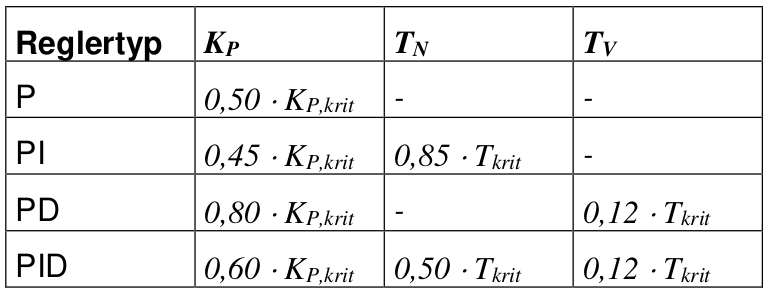
\includegraphics[width=\columnwidth]{images/stoergroessenaufschaltung.png}
\end{center}
Voraussetzung: Störgröße $z$ ist messbar und ihr Angriffsort bekannt. Das Störsignal wird über $F_{Sz}(s)$ direkt kompensiert, bevor es die Regelgröße auslenkt. Sehr schnelle Ausregelung ohne Stabilitätsverlust.
\end{tcolorbox}

\begin{tcolorbox}
\boxtitle{Vorsteuerung}
\begin{center}
  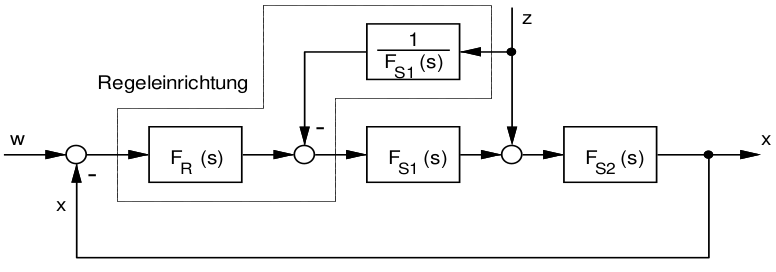
\includegraphics[width=\columnwidth]{images/vorsteuerung.png}
\end{center}
Wird eingesetzt, wenn kein optimaler Kompromiss zwischen Führungs- und Störverhalten möglich ist. Der Hauptregler wird auf gutes Störverhalten ausgelegt; der Vorsteuerfilter $F_{Rv}(s)$ beschleunigt das Folgen von $w(t)$.
\end{tcolorbox}

\begin{tcolorbox}
\boxtitle{Kaskadenregelung}
\begin{center}
  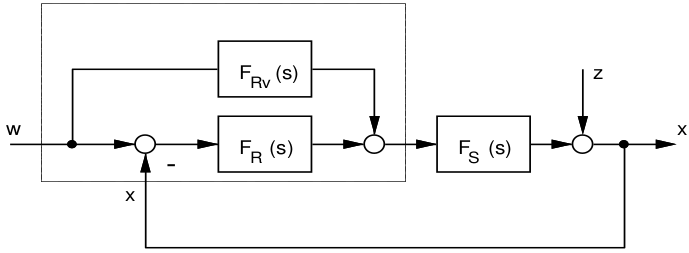
\includegraphics[width=\columnwidth]{images/kaskadenregelung.png}
\end{center}
Ineinandergeschachtelte Kreise. Der innere Hilfskreis ist deutlich schneller und regelt innere Störungen sofort aus. Inbetriebnahme erfolgt von innen nach außen.
\end{tcolorbox}

\begin{tcolorbox}
\boxtitle{Führungsgrößenfilter}
\begin{center}
  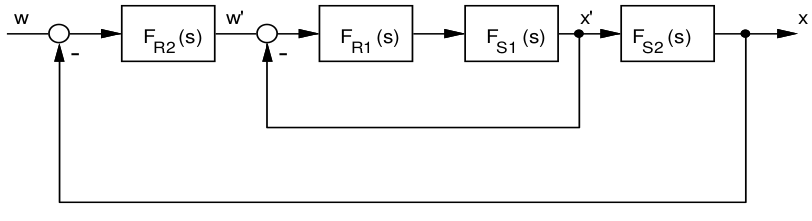
\includegraphics[width=0.9\columnwidth]{images/fuehrungsgroessenfilter.png}
\end{center}
Dominiert eine Nullstelle den geschlossenen Kreis, kommt es zu hohem Überschwingen. Ein vorgeschaltetes $PT_1$-Filter kompensiert diese Nullstelle exakt.
\end{tcolorbox}

\begin{tcolorbox}
\boxtitle{Anti-Windup (Grundprinzip)}
Bei Stellgrößenbegrenzung und I-Anteil läuft der Integrator unbegrenzt weiter (Windup), was zu extremem Überschwingen führt. Lösung: Begrenzung oder Anhalten des I-Anteils, sobald die Stellgrenze erreicht ist.
\end{tcolorbox}

\section{Digitale Regelungstechnik (Grundlagen)}

\subsection{Arbeitsweise realer Abtastsysteme}
\begin{tcolorbox}
\boxtitle{Signalpfad eines digitalen Regelkreises}
Im digitalen Regelkreis werden zeitkontinuierliche Signale periodisch mit der Abtastzeit $T_A$ (bzw. $\omega_A = 2\pi/T_A$) abgetastet:
\begin{enumerate}
  \item \textbf{Anti-Aliasing-Filter:} Analoges Tiefpassfilter vor der Abtastung zur Einhaltung des Shannon-Theorems ($f_g < f_A/2$).
  \item \textbf{Abtastglied (Sampler):} Entnimmt äquidistante Abtastwerte $e(k T_A)$.
  \item \textbf{Analog-Digital-Wandler (ADW):} Wandelt die Spannung in ein $N$-Bit-Wort.
  \[
  \text{Auflösung: } LSB = \frac{U_{\text{FS}}}{2^N - 1} \approx \frac{U_{\text{FS}}}{2^N}
  \]
  Quantisierungsrauschen: maximaler Fehler $\pm \frac{1}{2} LSB$.
  \item \textbf{Digitalrechner / Mikrocontroller:} Berechnet den Regelalgorithmus in einer festen Interrupt-Zeitscheibe $T_A$.
  \item \textbf{Halteglied nullter Ordnung (ZOH):} Hält den berechneten Stellwert $u(k T_A)$ über das Intervall $T_A$ konstant:
  \[
  g_{h0}(t) = \sigma(t) - \sigma(t - T_A) \implies G_{h0}(s) = \frac{1 - e^{-s T_A}}{s}
  \]
\end{enumerate}
\end{tcolorbox}

\begin{center}
  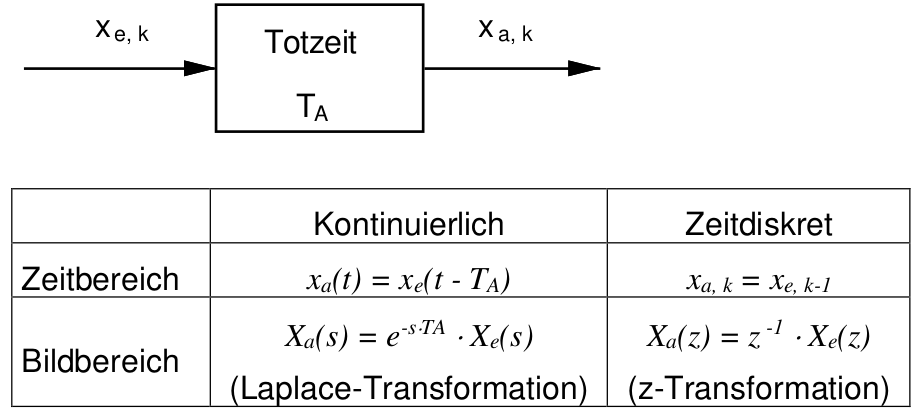
\includegraphics[width=\columnwidth]{images/abtastung_zeit.png}
\end{center}

\subsection{Die $z$-Transformation}
\begin{tcolorbox}
\boxtitle{Definition}
Für ein kausales diskretes Zeitsignal $\{f_k\} = \{f(k T_A)\}$ mit $f_k = 0$ für $k < 0$:
\[
F(z) = \mathcal{Z}\{f_k\} = \sum_{k=0}^\infty f_k \cdot z^{-k} \quad \text{mit } z = e^{s T_A}
\]
$z^{-1}$ entspricht im Zeitbereich einer Verzögerung um genau einen Abtastschritt $T_A$.
\end{tcolorbox}

\begin{tcolorbox}
\boxtitle{Korrespondenztabelle der $z$-Transformation}
\small
\begin{tabularx}{\columnwidth}{l X l}
\toprule
\textbf{Signal $f(t)$} & \textbf{Folge $f_k$} & \textbf{$z$-Transformierte $F(z)$} \\
\midrule
Impuls $\delta(t)$ & $\delta_k = (1, 0, 0, \dots)$ & $1$ \\[2pt]
Sprung $\sigma(t)$ & $\sigma_k = (1, 1, 1, \dots)$ & $\frac{z}{z-1}$ \\[3pt]
Rampe $t$ & $k \cdot T_A$ & $\frac{T_A z}{(z-1)^2}$ \\[3pt]
Parabel $t^2$ & $k^2 T_A^2$ & $\frac{T_A^2 z (z+1)}{(z-1)^3}$ \\[3pt]
Exp-Funktion $e^{-at}$ & $e^{-a k T_A}$ & $\frac{z}{z - e^{-a T_A}}$ \\[3pt]
$1 - e^{-at}$ & $1 - e^{-a k T_A}$ & $\frac{z (1 - e^{-a T_A})}{(z-1)(z - e^{-a T_A})}$ \\[3pt]
$t \cdot e^{-at}$ & $k T_A e^{-a k T_A}$ & $\frac{T_A z e^{-a T_A}}{(z - e^{-a T_A})^2}$ \\[3pt]
$\sin(\omega t)$ & $\sin(\omega k T_A)$ & $\frac{z \sin(\omega T_A)}{z^2 - 2z\cos(\omega T_A) + 1}$ \\[3pt]
$\cos(\omega t)$ & $\cos(\omega k T_A)$ & $\frac{z (z - \cos(\omega T_A))}{z^2 - 2z\cos(\omega T_A) + 1}$ \\[3pt]
$e^{-at}\sin(\omega t)$ & $e^{-ak T_A}\sin(\omega k T_A)$ & $\frac{z e^{-aT_A} \sin(\omega T_A)}{z^2 - 2z e^{-aT_A}\cos(\omega T_A) + e^{-2aT_A}}$ \\[3pt]
$e^{-at}\cos(\omega t)$ & $e^{-ak T_A}\cos(\omega k T_A)$ & $\frac{z (z - e^{-aT_A}\cos(\omega T_A))}{z^2 - 2z e^{-aT_A}\cos(\omega T_A) + e^{-2aT_A}}$ \\
\bottomrule
\end{tabularx}
\end{tcolorbox}

\begin{tcolorbox}
\boxtitle{Rechenregeln der $z$-Transformation}
\small
\begin{itemize}
  \item \textbf{Linearität:} $\mathcal{Z}\{a f_{1k} + b f_{2k}\} = a F_1(z) + b F_2(z)$
  \item \textbf{Rechtsverschiebung (Verzögerung um $n$ Schritte):}
  \[
  \mathcal{Z}\{f_{k-n}\} = z^{-n} \cdot F(z) \quad (\text{für } f_k = 0 \text{ bei } k < 0)
  \]
  \item \textbf{Linksverschiebung (Vorauseilung):}
  \[
  \mathcal{Z}\{f_{k+n}\} = z^n \left[ F(z) - \sum_{i=0}^{n-1} f_i z^{-i} \right]
  \]
  \item \textbf{Rückwärtsdifferenz:}
  \[
  \mathcal{Z}\{f_k - f_{k-1}\} = \frac{z-1}{z} F(z) - f_{-1}
  \]
  \item \textbf{Vorwärtsdifferenz:}
  \[
  \mathcal{Z}\{f_{k+1} - f_k\} = (z-1) F(z) - f_0 z
  \]
  \item \textbf{Dämpfungssatz:}
  \[
  \mathcal{Z}\{f_k \cdot e^{-a k T_A}\} = F(z \cdot e^{a T_A})
  \]
  \item \textbf{Summensatz:}
  \[
  \mathcal{Z}\left\{ \sum_{\nu=0}^k f_\nu \right\} = \frac{z}{z-1} \cdot F(z)
  \]
  \item \textbf{Differentiation im Bildbereich:}
  \[
  \mathcal{Z}\{k \cdot f_k\} = -z \cdot \frac{d F(z)}{dz}
  \]
  \item \textbf{Faltungssatz:}
  \[
  \mathcal{Z}\{f_k * g_k\} = \mathcal{Z}\left\{ \sum_{\nu=0}^k f_\nu g_{k-\nu} \right\} = F(z) \cdot G(z)
  \]
  \item \textbf{Anfangswertsatz:}
  \[
  f_0 = f(t \to 0) = \lim_{z \to \infty} F(z)
  \]
  \item \textbf{Endwertsatz:}
  \[
  f_\infty = \lim_{k \to \infty} f_k = \lim_{z \to 1} (z - 1) \cdot F(z)
  \]
  (Voraussetzung: Alle Pole von $(z-1)F(z)$ liegen strikt innerhalb des Einheitskreises).
\end{itemize}
\end{tcolorbox}

\subsection{Stabilität im $z$-Bereich}
\begin{tcolorbox}
Ein zeitdiskretes LTI-System mit der $z$-Übertragungsfunktion $F(z)$ ist genau dann \textbf{BIBO-stabil}, wenn alle Pole $z_{P,i}$ von $F(z)$ \textbf{strikt innerhalb des Einheitskreises} der komplexen $z$-Ebene liegen:
\[
|z_{P,i}| < 1 \quad \forall i = 1, \dots, n
\]
\textbf{Abbildung der $s$-Ebene in die $z$-Ebene:}
Mit $s = \sigma + j\omega$ und $z = e^{s T_A}$:
\[
z = e^{(\sigma + j\omega) T_A} = e^{\sigma T_A} \cdot e^{j \omega T_A} \implies |z| = e^{\sigma T_A}, \quad \angle z = \omega T_A
\]
\begin{itemize}
  \item $\sigma < 0$ (linke $s$-Halbebene, stabil) $\implies |z| < 1$ (Inneres des Einheitskreises).
  \item $\sigma = 0$ (Imaginärachse, Stabilitätsgrenze) $\implies |z| = 1$ (Einheitskreislinie).
  \item $\sigma > 0$ (rechte $s$-Halbebene, instabil) $\implies |z| > 1$ (Äußeres des Einheitskreises).
  \item $0 < z < 1$ (positive reelle Achse): Rein aperiodisches Verhalten ($D \ge 1$, kein Überschwingen).
  \item $-1 < z < 0$ (negative reelle Achse): Oszillation mit der halben Abtastfrequenz $\omega = \frac{\pi}{T_A} = \frac{\omega_A}{2}$ (Nyquist-Grenze, da $(-1)^k$ alterniert).
  \item $z = 0$ (Ursprung): Vollkommene Dämpfung / Deadbeat (Antwort klingt in endlich vielen Schritten exakt ab).
  \item $z = 1$: Integrator ($s = 0$).
\end{itemize}
\end{tcolorbox}

\subsection{Näherungsverfahren zur Transformation $s \to z$}
\begin{tcolorbox}
Da der exakte Zusammenhang $z = e^{s T_A}$ für gebrochen rationale Funktionen nicht rational ist, verwendet man Näherungen:

\textbf{1. Rückwärtsdifferenzenquotient:}
\[
s \approx \frac{1 - z^{-1}}{T_A} = \frac{z - 1}{T_A \cdot z}
\]
Ersetzung: $F(z) = F(s)\big|_{s = \frac{z-1}{T_A z}}$.
Stabile $s$-Systeme bleiben immer stabil. Allerdings können instabile $s$-Pole fälschlich in den Einheitskreis abgebildet werden.

\textbf{2. Vorwärtsdifferenzenquotient (Euler):}
\[
s \approx \frac{z - 1}{T_A}
\]
Ersetzung: $F(z) = F(s)\big|_{s = \frac{z-1}{T_A}}$.
Sehr einfach zu berechnen. Nachteil: Stabile $s$-Systeme können im $z$-Bereich instabil werden!

\textbf{3. Tustinsche Formel (Bilineartransformation):}
\[
s \approx \frac{2}{T_A} \cdot \frac{z - 1}{z + 1}
\]
Bildet die gesamte linke $s$-Halbebene bijektiv auf das Innere des Einheitskreises ab. Stabilität bleibt exakt erhalten.
\textbf{Frequenzverzerrung (Prewarping):}
\[
\omega_w = \frac{2}{T_A} \tan\left( \frac{\omega T_A}{2} \right)
\]
\end{tcolorbox}

\subsection{Rechenalgorithmus aus $F(z)$}
\begin{tcolorbox}
\boxtitle{Vorgehensweise zur Bestimmung der Differenzengleichung}
Gegeben ist die $z$-Übertragungsfunktion $F(z) = \frac{X_a(z)}{X_e(z)}$:
\begin{enumerate}
  \item Zähler und Nenner durch die höchste Potenz von $z$ teilen, sodass nur Terme $z^0, z^{-1}, z^{-2}, \dots$ verbleiben.
  \[
  F(z) = \frac{b_0 + b_1 z^{-1} + \dots + b_m z^{-m}}{a_0 + a_1 z^{-1} + \dots + a_n z^{-n}}
  \]
  \item Ausmultiplizieren:
  \[
  X_a(z) \cdot \sum a_i z^{-i} = X_e(z) \cdot \sum b_i z^{-i}
  \]
  \item Rücktransformation in den Zeitbereich ($z^{-i} \leftrightarrow$ Verzögerung um $i$ Abtastschritte):
  \[
  a_0 x_{a,k} + a_1 x_{a,k-1} + \dots = b_0 x_{e,k} + b_1 x_{e,k-1} + \dots
  \]
  \item Auflösen nach dem aktuellen Stellwert $x_{a,k}$:
  \[
  x_{a,k} = \frac{1}{a_0} \left[ \sum_{i=0}^m b_i x_{e,k-i} - \sum_{j=1}^n a_j x_{a,k-j} \right]
  \]
\end{enumerate}
\textbf{Beispiel:}
\[
F(z) = \frac{2z + 4}{8z - 5} = \frac{2 + 4 z^{-1}}{8 - 5 z^{-1}}
\]
\[
8 x_{a,k} - 5 x_{a,k-1} = 2 x_{e,k} + 4 x_{e,k-1}
\]
\[
\implies x_{a,k} = 0{,}25 \cdot x_{e,k} + 0{,}50 \cdot x_{e,k-1} + 0{,}625 \cdot x_{a,k-1}
\]
\end{tcolorbox}

\begin{tcolorbox}
\boxtitle{Implementierung in Programmcode (C)}
\begin{lstlisting}
while (1) {
    wait_timerinterrupt(TA); // Abtastzeit warten
    
    // Alte Werte weiterschieben
    xaalt1 = xa;
    xealt1 = xe;
    
    // Eingangswert einlesen
    input(xe);
    
    // Differenzengleichung berechnen
    xa = 0.25 * xe + 0.50 * xealt1 + 0.625 * xaalt1;
    
    // Stellwert ausgeben
    output(xa);
}
\end{lstlisting}
\end{tcolorbox}

\subsection{Kausalität \& Signalflussplan im Diskreten}
\begin{tcolorbox}
\textbf{Kausalitätsbedingung:}\\[2pt]
Ein diskretes System ist als physikalischer Rechenalgorithmus genau dann realisierbar, wenn der Nennergrad mindestens so groß ist wie der Zählergrad:
\[
\deg(\text{Zähler}) \le \deg(\text{Nenner}) \iff m \le n
\]
\begin{itemize}
  \item $m < n$: Streng kausal (Ausgang hängt nur von vergangenen Eingängen ab, Verzögerung um $(n-m) T_A$).
  \item $m = n$: Kausal (Ausgang hängt auch vom aktuellen Eingang $x_{e,k}$ ab).
  \item $m > n$: Nicht kausal (erfordert zukünftige Werte $x_{e,k+1} \implies$ nicht echtzeitfähig!).
\end{itemize}
\end{tcolorbox}

\section{Zeitdiskreter Reglerentwurf}

\subsection{Quasi-kontinuierlicher Reglerentwurf}
\begin{tcolorbox}
Gültigkeitsbereich: Bei sehr kleinen Abtastzeiten $T_A$ im Vergleich zur dominierenden Systemzeitkonstante $T_{\text{dom}}$:
\[
T_A \le \frac{1}{10} \dots \frac{1}{20} \cdot T_{\text{dom}}
\]
\textbf{Vorgehen:}
\begin{enumerate}
  \item Kontinuierlicher Entwurf des Reglers $F_R(s)$ mit klassischen Methoden (Bode-Verfahren, Betragsoptimum, Ziegler-Nichols).
  \item Diskretisierung des fertigen Reglers mit der Tustin-Transformation oder dem Rückwärtsdifferenzenquotienten.
\end{enumerate}
\end{tcolorbox}

\subsection{Exakte zeitdiskrete Modellbildung der Strecke (ZOH-Transformation)}
\begin{tcolorbox}
\boxtitle{Strecke mit Halteglied 0. Ordnung ($G_{h0}$)}
Wird eine kontinuierliche Strecke $F_S(s)$ über ein Abtast- und Halteglied angesteuert, berechnet sich die exakte zeitdiskrete Übertragungsfunktion $F_{S0}(z)$ zu:
\begin{align*}
F_{S0}(z) &= \mathcal{Z}\{ G_{h0}(s) \cdot F_S(s) \} = \mathcal{Z}\left\{ \frac{1 - e^{-s T_A}}{s} \cdot F_S(s) \right\} \\
&= (1 - z^{-1}) \cdot \mathcal{Z}\left\{ \frac{F_S(s)}{s} \right\} = \frac{z - 1}{z} \cdot \mathcal{Z}\left\{ \frac{F_S(s)}{s} \right\}
\end{align*}
\textbf{Standard-Streckentypen:}
\begin{itemize}
  \item \textbf{PT$_1$-Strecke} $F_S(s) = \frac{K_S}{1 + s T_1}$:
  \[
  F_{S0}(z) = K_S \cdot \frac{1 - e^{-T_A/T_1}}{z - e^{-T_A/T_1}}
  \]
  \item \textbf{I-Strecke} $F_S(s) = \frac{K_I}{s}$:
  \[
  F_{S0}(z) = \frac{K_I \cdot T_A}{z - 1}
  \]
  \item \textbf{IT$_1$-Strecke} $F_S(s) = \frac{K_I}{s (1 + s T_1)}$:
  \[
  F_{S0}(z) = K_I \left[ \frac{T_A}{z - 1} - \frac{T_1 (1 - e^{-T_A/T_1})}{z - e^{-T_A/T_1}} \right]
  \]
\end{itemize}
\end{tcolorbox}

\subsection{Wurzelortskurven im Zeitdiskreten}
\begin{tcolorbox}
\boxtitle{WOK in der $z$-Ebene}
Für die geometrische Konstruktion der WOK gelten \textbf{exakt dieselben algebraischen Regeln} wie im Kontinuierlichen (Start in offenen Polen bei $K=0$, Ende in Nullstellen für $K \to \infty$, Wurzelschwerpunkt, Asymptoten, reelle Achsenbelegung).\\[3pt]
\textbf{Wesentliche Unterschiede zum $s$-Bereich:}
\begin{itemize}
  \item \textbf{Stabilitätsgrenze:} Ist \textbf{nicht} die Imaginärachse, sondern der \textbf{Einheitskreis $|z| = 1$}.
  \item Pole mit Dämpfung $D \ge 1$ (kein Schwingen) liegen ausschließlich auf der positiven reellen Achse im Intervall $0 \le z < 1$.
  \item Pole auf der negativen reellen Achse $(-1 < z < 0)$ oszillieren mit der Nyquist-Frequenz $\omega = \pi / T_A$.
  \item \textbf{Kritische Verstärkung $K_{\text{krit}}$:} Ergibt sich aus den Schnittpunkten der WOK mit der Einheitskreislinie $|z| = 1$.
  \item \textbf{Schwingfrequenz an der Stabilitätsgrenze:}
  \[
  \omega_{\text{krit}} = \frac{\varphi_{\text{Pol}}}{T_A} \quad \text{mit } z = 1 \cdot e^{j \varphi_{\text{Pol}}}
  \]
  \item \textbf{Dämpfung $D$:} Kurven konstanter Dämpfung $D$ sind logarithmische Spiralen im Einheitskreis.
\end{itemize}
\end{tcolorbox}

\subsection{Dead-Beat Regler (Kompensationsregler)}

\begin{tcolorbox}
\boxtitle{Grundgleichungen des Kompensationsreglers}
Führungsübertragungsfunktion des Regelkreises mit Messglied $F_M(z)$:
\[
F_{\text{RK}}(z) = \frac{F_R(z) \cdot F_S(z)}{1 + F_R(z) \cdot F_S(z) \cdot F_M(z)} \stackrel{!}{=} F_w(z)
\]
Auflösen nach der gesuchten Reglerübertragungsfunktion $F_R(z)$:
\[
F_R(z) = \frac{F_w(z)}{F_S(z) \cdot [1 - F_w(z) \cdot F_M(z)]}
\]
\textbf{Zulässigkeitsbedingungen:}
\begin{enumerate}
  \item Die Strecke $F_S(z)$ darf keine instabilen Pole oder Nullstellen außerhalb des Einheitskreises besitzen (dürfen nicht gekürzt werden!).
  \item Realisierbarkeit: Der Polüberschuss der Wunschfunktion muss mindestens so groß sein wie der der Strecke:
  \[
  PÜ(F_w) \ge PÜ(F_S)
  \]
\end{enumerate}
\end{tcolorbox}

\begin{tcolorbox}
\boxtitle{Klassischer Deadbeat-Entwurf}
Forderung: Einschwingen auf den Sollwert in minimaler Zeit ($n + d$ Abtastschritte, $n$: Streckenordnung, $d$: Totzeit):
\[
F_w(z) = \frac{1}{z^{n+d}} = z^{-(n+d)}
\]
\textbf{Stationäre Verstärkung einer $z$-Übertragungsfunktion:}
\[
K = F(z = 1) = F(1) = \frac{\sum_{i=0}^m b_i}{\sum_{j=0}^n a_j}
\]
\end{tcolorbox}

\begin{tcolorbox}
\boxtitle{Erzwingen eines Reglers mit $I$-Anteil}
Ohne $I$-Anteil führt jede Modellunsicherheit oder Laststörung zu einer bleibenden Regelabweichung ($e_\infty \ne 0$).\\[3pt]
\textbf{Bedingung für Pol bei $z = 1$ im Regler:}
Der Nenner von $F_R(z)$ muss für $z = 1$ verschwinden:
\[
1 - F_w(1) \cdot F_M(1) = 0 \implies F_w(1) = \frac{1}{F_M(1)} = \frac{1}{K_M}
\]
\textbf{Lösung:} Einfügen eines Vorfilters $K_F = K_M$ im Führungszweig. Dadurch gilt für die Gesamtführung $K_w = 1$, die stationäre Regeldifferenz wird exakt $e(\infty) = 0$, und $F_R(z)$ erhält zwingend einen integralen Pol bei $z = 1$.
\end{tcolorbox}

\begin{tcolorbox}
\boxtitle{Vermeidung von Zwischenabtast-Oszillationen (Ripples)}
\textbf{Ursache:} Die Übertragungsfunktion vom Sollwert $w$ zur Stellgröße $u$ lautet:
\[
F_{wu}(z) = \frac{U(z)}{W(z)} = \frac{F_w(z)}{F_S(z)}
\]
Alle Zählernullstellen der Strecke $F_S(z)$ werden zu Polen von $F_{wu}(z)$! Liegen diese bei negativen Werten (z.\,B. nahe $-1$), so schwingt die Stellgröße $u_k$ mit der halben Abtastfrequenz und regt die analoge Strecke zwischen den Abtastpunkten zu Dauerschwingungen an (\textit{Hidden Oscillations}).\\[3pt]
\textbf{Abhilfe durch Hilfsfunktion $F_H(z)$:}
Erweiterung der Wunschübertragungsfunktion:
\[
F_{w,\text{neu}}(z) = F_w(z) \cdot F_H(z)
\]
\textbf{Bedingungen an $F_H(z)$:}
\begin{enumerate}
  \item $F_H(z)$ enthält im Zähler exakt die kritischen Nullstellen von $F_S(z)$, um die Pole in $F_{wu}$ zu kürzen.
  \item Statische Verstärkung $F_H(1) = 1$ (keine Verfälschung des Endwerts).
  \item Polüberschuss $PÜ(F_H) = 0$ (gleicher Zähler- und Nennergrad).
\end{enumerate}
\end{tcolorbox}

\begin{tcolorbox}
\boxtitle{Alternative gestufte Wunschfunktionen}
Zur Schonung von Stellgliedern und Vermeidung extremer Stellgrößenspitzen kann der Sollwertsprung in $N$ Teilschritten angefahren werden (z.\,B. $0\% \to 50\% \to 80\% \to 100\%$):
\[
x_{a,k} = \{0, a_1, a_2, 1, 1, \dots\}
\]
\[
F_w(z) = a_1 z^{-1} + (a_2 - a_1) z^{-2} + (1 - a_2) z^{-3}
\]
\end{tcolorbox}

\begin{tcolorbox}
\boxtitle{Stellgrößenbeschränkungen beim Deadbeat-Regler}
Geht die Stellgröße $u_k$ in die Sättigung ($u_{\max}$), ist die Linearitätsannahme verletzt $\implies$ stark verlängertes Einschwingen.\\[2pt]
\textbf{Gegenmaßnahme:} Rückrechnung der maximal zulässigen Führungsgröße $w_{\text{korr},k}$ aus dem Regelalgorithmus für den aktuellen Schritt, sodass $u_k = u_{\max}$ exakt eingehalten wird.
\end{tcolorbox}

\section{Modellierung mechatronischer Systeme}

\subsection{Systematik der Modellbildung}
\begin{tcolorbox}
\boxtitle{Vier Phasen der Modellierung}
\begin{enumerate}
  \item \textbf{Ziel bestimmen:} Reglerentwurf, Simulation, Belastungsanalyse? Statisch oder dynamisch? Geforderte Modellgenauigkeit?
  \item \textbf{Modellstruktur festlegen:} Ein- und Ausgangsgrößen definieren, Systemgrenzen ziehen, Zerlegung in Teilsysteme (elektrisch, mechanisch, thermisch).
  \item \textbf{Parameter bestimmen:} Aus Datenblättern, Messungen im Arbeitspunkt oder Identifikationsverfahren.
  \item \textbf{Modellvalidierung:} Plausibilitätsprüfungen (Einheiten, Vorzeichen) und Vergleich der Simulation mit realen Messdaten.
\end{enumerate}
\end{tcolorbox}

\subsection{Modellierung am Beispiel Drosselklappe}

\begin{tcolorbox}
\boxtitle{1. Elektrisches Teilsystem (Gleichstrommotor)}
Maschengleichung des Ankerkreises:
\[
u_A(t) = R_A \cdot i_A(t) + L_A \cdot \frac{di_A(t)}{dt} + u_{\text{EMK}}(t)
\]
Elektromotorische Gegenkraft (EMK):
\[
u_{\text{EMK}}(t) = k_{\text{EMK}} \cdot \omega_M(t) = k_{\text{EMK}} \cdot k_G \cdot \dot{\varphi}(t)
\]
Elektromagnetisches Motormoment:
\[
M_{\text{Mot}}(t) = k_M \cdot i_A(t)
\]
\end{tcolorbox}

\begin{tcolorbox}
\boxtitle{2. Mechanisches Teilsystem (Klappenmechanik)}
Drallsatz um die Drehachse der Drosselklappe:
\[
J \cdot \ddot{\varphi}(t) + d \cdot \dot{\varphi}(t) + M_F(\varphi) + M_{\text{Reib}}(\dot{\varphi}) = M_{\text{Klappe}}(t)
\]
mit dem Antriebsmoment $M_{\text{Klappe}} = k_G \cdot M_{\text{Mot}}$:
\begin{itemize}
  \item $J$: Gesamt-Massenträgheitsmoment auf Klappenachse bezogen.
  \item $d$: Viskoser Dämpfungsbeiwert.
  \item $M_F(\varphi) = c_F \cdot (\varphi(t) - \varphi_0)$: Rückstellmoment der Rückholfeder (Fail-Safe Ruhelage $\varphi_0$).
  \item $M_{\text{Reib}}$: Reibung (Coulomb-Gleitreibung und Haftreibung).
  \item $k_G$: Übersetzungsverhältnis des Getriebes ($k_G = \omega_M / \dot{\varphi}$).
\end{itemize}
\end{tcolorbox}

\begin{tcolorbox}
\boxtitle{3. Modellvereinfachungen für den Reglerentwurf}
\begin{itemize}
  \item \textbf{Elektrische Zeitkonstante:} Da $T_{\text{el}} = \frac{L_A}{R_A} \ll T_{\text{mech}}$, wird die Ankerinduktivität für den linearen Reglerentwurf meist vernachlässigt ($L_A \approx 0$):
  \[
  i_A(t) \approx \frac{u_A(t) - k_{\text{EMK}} \cdot k_G \cdot \dot{\varphi}(t)}{R_A}
  \]
  \item \textbf{Vernachlässigung von Feder und Reibung:}
  Für schnelle Lageänderungen dominiert das Trägheitsmoment $J \ddot{\varphi}$. Das System nähert sich einem idealen $IT_1$-Verhalten von Eingangsspannung $u_A$ zu Klappenwinkel $\varphi$:
  \[
  F_S(s) = \frac{\Phi(s)}{U_A(s)} \approx \frac{K}{s (1 + s T_{\text{mech}})}
  \]
  mit $T_{\text{mech}} = \frac{J \cdot R_A}{d \cdot R_A + k_M \cdot k_{\text{EMK}} \cdot k_G^2}$.
\end{itemize}
\end{tcolorbox}

\begin{tcolorbox}
\boxtitle{Plausibilitätsprüfungen}
\begin{itemize}
  \item Vorzeichen der Kennlinien prüfen (z.\,B. Reibmoment wirkt immer der Bewegungsrichtung entgegen: $\text{sign}(\dot{\varphi})$).
  \item Federmoment muss im stromlosen Zustand größer sein als die Reibung ($M_F > M_{\text{Reib}}$), damit Fail-Safe gesichert ist.
  \item Maximales Motormoment muss Feder- und Reibmoment sicher überwinden: $k_M \cdot I_{\max} \cdot k_G > M_F + M_{\text{Reib}}$.
\end{itemize}
\end{tcolorbox}

\section{Praktische Aspekte digitaler Regler}

\subsection{Pulsweitenmodulation (PWM)}
\begin{tcolorbox}
\boxtitle{Funktionsprinzip}
Zur verlustarmen Leistungssteuerung wird die feste Versorgungsspannung $U_0$ mit konstanter Schaltfrequenz $f_{\text{PWM}} = \frac{1}{T_{\text{PWM}}}$ getaktet.\\[2pt]
\textbf{Tastgrad (Duty Cycle):}
\[
v = \frac{T_{\text{ein}}}{T_{\text{PWM}}} \in [0, 1] \quad (\text{bzw. } 0 \dots 100\%)
\]
\textbf{Mittelwertbildung} (Trägheit von Motor oder Last $\gg T_{\text{PWM}}$):
\begin{align*}
\text{Mittlere Spannung:} \quad &\bar{u} = v \cdot U_0 \\
\text{Mittlerer Strom:} \quad &\bar{i} = v \cdot I_0 \\
\text{Mittleres Drehmoment:} \quad &\bar{M} = v \cdot M_0
\end{align*}
\textbf{Vorteil:} Schalter (MOSFETs) sind voll durchgeschaltet oder gesperrt $\implies$ minimale Verlustleistung im Stellglied!
\end{tcolorbox}

\begin{tcolorbox}
\boxtitle{H-Brücken-Ansteuerung (4-Quadrantenbetrieb)}
Ermöglicht Drehrichtungsumkehr und aktives Bremsen:
\begin{center}
\small
\begin{tabularx}{\columnwidth}{l c c c c c}
\toprule
\textbf{Zustand} & \textbf{DIR} & \textbf{PWM} & \textbf{ENA} & \textbf{OUT1} & \textbf{OUT2} \\
\midrule
Antrieb pos. (Puls) & L & H & H & L & H \\
Antrieb neg. (Puls) & H & H & H & H & L \\
Bremse low-side (Pause) & L & L & H & L & L \\
Bremse high-side (Pause) & H & L & H & H & H \\
Freilauf / Abschaltung & X & X & L & Z & Z \\
\bottomrule
\end{tabularx}
\end{center}
\scriptsize ($H$: High, $L$: Low, $X$: beliebig, $Z$: hochohmig/gesperrt).
\end{tcolorbox}

\subsection{Integer- und Festkomma-Arithmetik}
\begin{tcolorbox}
\boxtitle{Gründe für Festkomma-Arithmetik}
Einfache Mikrocontroller besitzen keine Gleitkomma-Hardware (FPU). Software-Gleitkomma erhöht Codeumfang und Rechenzeit drastisch.
\end{tcolorbox}

\begin{tcolorbox}
\boxtitle{Festkomma-Skalierung (Q-Format)}
Eine Fließkommazahl $x$ wird durch Multiplikation mit $2^Q$ als Ganzzahl dargestellt:
\[
x_{\text{int}} = \text{round}(x \cdot 2^Q)
\]
\begin{itemize}
  \item \textbf{Addition / Subtraktion:} Direkt möglich (gleiches $Q$-Format vorausgesetzt).
  \item \textbf{Multiplikation:}
  \[
  z_{\text{int}} = (x_{\text{int}} \cdot y_{\text{int}}) \gg Q \quad (\text{Rechtsshift um } Q \text{ Bits})
  \]
  \item \textbf{Zwischenergebnisse:} Immer in doppelter Bitbreite berechnen (z.\,B. \texttt{int16\_t} $\times$ \texttt{int16\_t} $\to$ \texttt{int32\_t}).
\end{itemize}
\end{tcolorbox}

\begin{tcolorbox}
\boxtitle{Typische numerische Gefahren}
\begin{enumerate}
  \item \textbf{Zahlenbereichsüberlauf (Overflow):}
  Führt bei Zweierkomplement zu Vorzeichenumkehr (z.\,B. $+127 + 1 = -128$ bei \texttt{int8}). $\implies$ \textbf{Sättigungsarithmetik} einsetzen!
  \item \textbf{Kürzungsfehler bei Division:}
  Eine Division vor einer Multiplikation kann ganzzahlig zu 0 führen. $\implies$ \textbf{Immer erst multiplizieren, dann dividieren!}
  \[
  \text{Falsch: } (a / b) * c \qquad \text{Richtig: } (a * c) / b
  \]
  \item \textbf{Quantisierungsfehler:} Bei kleinen Signalen führt Rundung zu Totzonen oder Grenzschwingungen.
\end{enumerate}
\end{tcolorbox}

\subsection{Anti-Windup-Algorithmen}
\begin{tcolorbox}
\boxtitle{Das Windup-Problem}
Bei Begrenzung der Stellgröße (z.\,B. Spannung $U_{\max}$, maximaler PWM-Wert) kann das System dem Sollwert nicht sofort folgen. Ein integrierender Regler (I-Anteil) summiert die Regeldifferenz weiter auf (\textit{Windup}). Beim Erreichen des Sollwerts ist der I-Anteil stark überladen und verursacht enormes Überschwingen.
\end{tcolorbox}

\begin{tcolorbox}
\boxtitle{1. Clamping (Integrator-Verriegelung)}
Das Aufintegrieren wird blockiert, wenn:
\begin{itemize}
  \item die Stellgröße in der Sättigung ist ($|u| \ge u_{\max}$) \textbf{und}
  \item die Regeldifferenz $e$ das gleiche Vorzeichen wie $u$ hat (was die Sättigung weiter vertiefen würde).
\end{itemize}
\end{tcolorbox}

\begin{tcolorbox}
\boxtitle{2. Back-Calculation (Rückrechnung)}
Die Differenz zwischen unbegrenzter Stellgröße $u$ und begrenztem Stellwert $u_{\text{sat}}$ wird über eine Nachführkonstante $\frac{1}{T_t}$ auf den Integrator rückgeführt:
\[
\dot{x}_I(t) = e(t) - \frac{1}{T_t} \cdot [u(t) - u_{\text{sat}}(t)]
\]
Im Zeitdiskreten (mit Abtastzeit $T_A$):
\[
x_{I,k} = x_{I,k-1} + T_A \cdot e_k - \frac{T_A}{T_t} \cdot (u_k - u_{\text{sat},k})
\]
Typische Wahl: $T_t \approx T_I$ (Nachstellzeit des I-Anteils).
\end{tcolorbox}

\subsection{Task-Scheduling \& Echtzeitanforderungen}
\begin{tcolorbox}
\boxtitle{Zustände eines Tasks}
\begin{itemize}
  \item \textbf{Running:} Task wird gerade von der CPU ausgeführt.
  \item \textbf{Ready:} Task ist ausführbereit und wartet auf CPU-Zuteilung durch den Scheduler.
  \item \textbf{Blocked / Waiting:} Task wartet auf ein externes Ereignis (Timer-Interrupt, Datenempfang).
\end{itemize}
\end{tcolorbox}

\begin{tcolorbox}
\boxtitle{Echtzeit-Anforderung für Regler}
\begin{itemize}
  \item Die Theorie zeitdiskreter Systeme setzt eine \textbf{strikt konstante Abtastzeit $T_A$} voraus.
  \item Zeitschwankungen (\textit{Jitter}) wirken wie additives Rauschen und Phasenverlust $\implies$ Destabilisierung!
  \item \textbf{Realisierung:} Der Regler-Task muss über einen \textbf{Hardware-Timer-Interrupt} mit \textbf{höchster Priorität} (preemptive) ausgeführt werden. Längere Hintergrundaufgaben (Display, Logging, Kommunikation) laufen mit niedrigerer Priorität im Hintergrund.
\end{itemize}
\end{tcolorbox}

\section{Systembeschreibung im Zustandsraum}

\subsection{Allgemeine MIMO-Zustandsdarstellung}
\begin{tcolorbox}
\boxtitle{Zustandsdifferentialgleichung und Ausgangsgleichung}
Kontinuierliches Mehrgrößensystem (MIMO) mit Zustandsvektor $\vec{x}(t) \in \mathbb{R}^n$, Eingangsvektor $\vec{u}(t) \in \mathbb{R}^p$ und Ausgangsvektor $\vec{y}(t) \in \mathbb{R}^q$:
\begin{align*}
\dot{\vec{x}}(t) &= A \vec{x}(t) + B \vec{u}(t), \quad \vec{x}(0) = \vec{x}_0 \\
\vec{y}(t) &= C \vec{x}(t) + D \vec{u}(t)
\end{align*}
\begin{itemize}
  \item $A \in \mathbb{R}^{n \times n}$: Systemmatrix (beschreibt innere Dynamik)
  \item $B \in \mathbb{R}^{n \times p}$: Eingangsmatrix (Steuermatrix)
  \item $C \in \mathbb{R}^{q \times n}$: Ausgangsmatrix (Beobachtungsmatrix)
  \item $D \in \mathbb{R}^{q \times p}$: Durchgangsmatrix (direkter Durchgriff)
\end{itemize}
\end{tcolorbox}

\begin{center}
  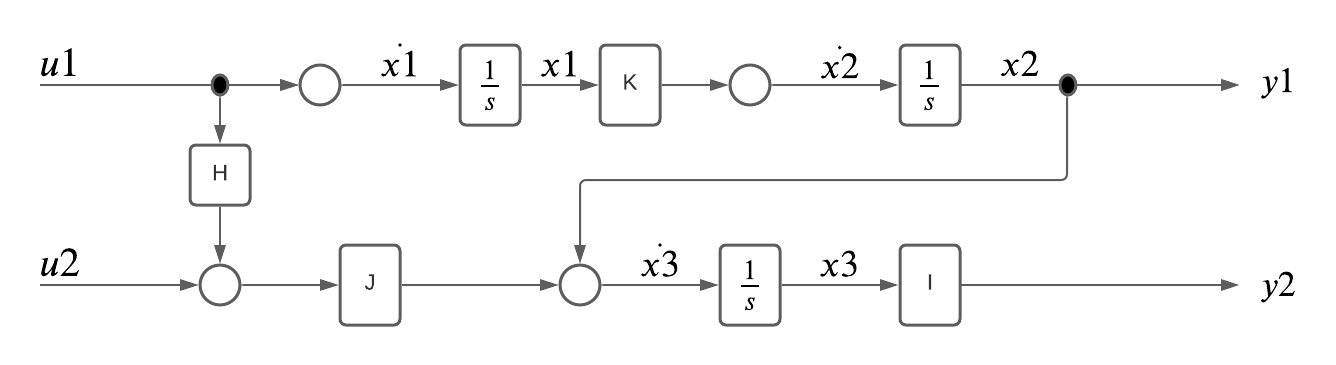
\includegraphics[width=\columnwidth]{images/zustandsraum_bsb.png}
\end{center}

\begin{tcolorbox}
\boxtitle{Pole des Systems / Eigenwerte von $A$}
Die Eigenwerte der Systemmatrix $A$ sind identisch mit den Polen des Systems:
\[
\det(A - sI) \stackrel{!}{=} 0 \implies \text{charakteristisches Polynom}
\]
Das System ist asymptotisch stabil, wenn alle Eigenwerte $\lambda_i$ von $A$ einen echt negativen Realteil besitzen ($\text{Re}\{\lambda_i\} < 0$).
\end{tcolorbox}

\subsection{Polfestlegung durch Zustandsrückführung}
\begin{tcolorbox}
\boxtitle{Vollständige Zustandsrückführung}
\begin{center}
  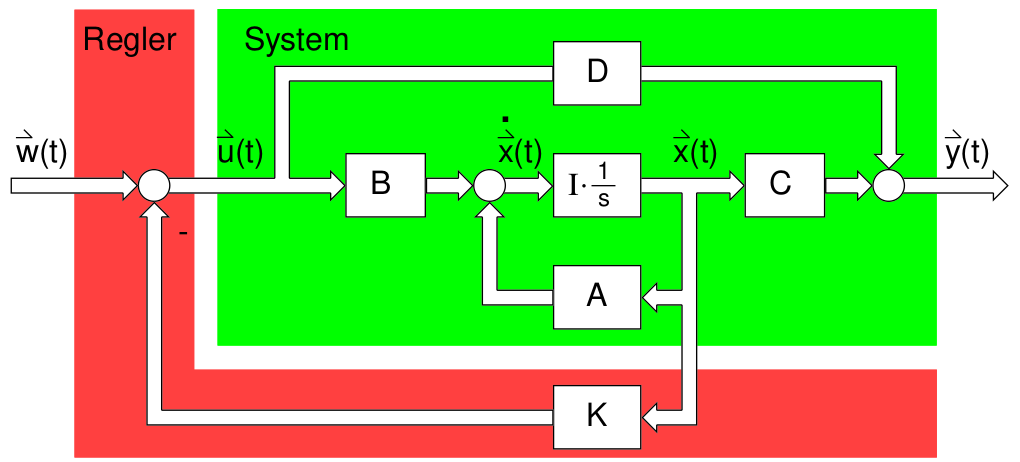
\includegraphics[width=\columnwidth]{images/zustandsrueckfuehrung.png}
\end{center}
Rückführung aller Zustandsgrößen über die Rückführmatrix $K \in \mathbb{R}^{p \times n}$:
\[
\vec{u}(t) = \vec{w}(t) - K \cdot \vec{x}(t)
\]
Einsetzen in die Zustandsdifferentialgleichung:
\[
\dot{\vec{x}}(t) = (A - B K) \vec{x}(t) + B \vec{w}(t)
\]
\textbf{Neue geschlossene Systemmatrix:}
\[
A_{\text{RK}} = A - B K
\]
\end{tcolorbox}

\begin{tcolorbox}
\boxtitle{Polplatzierung durch Koeffizientenvergleich}
Ist das System vollständig steuerbar ($\text{Rang}[B, AB, \dots, A^{n-1}B] = n$), so können durch freie Wahl der Koeffizienten von $K$ alle $n$ Pole des geschlossenen Systems \textbf{vollkommen frei} platziert werden:
\[
\det(A_{\text{RK}} - sI) = \det(A - BK - sI) \stackrel{!}{=} P_{\text{soll}}(s)
\]
mit dem gewünschten charakteristischen Polynom:
\[
P_{\text{soll}}(s) = \prod_{i=1}^n (s - s_{P,\text{soll},i}) = s^n + p_{n-1} s^{n-1} + \dots + p_0
\]
Durch Koeffizientenvergleich der Potenzen von $s$ werden die Elemente des Rückführvektors $K = [k_1, k_2, \dots, k_n]$ direkt bestimmt.
\end{tcolorbox}


\end{document}
